\documentclass[a4paper,oneside]{article}
\usepackage{indentfirst}
\usepackage{graphicx}
\usepackage{listings}
\usepackage{newtxtext,newtxmath}
\usepackage[top=0.7in, bottom=0.7in, left = 0.7in, right = 0.7in]{geometry}
\usepackage{enumitem}
\usepackage{caption}
\setlist{nolistsep}
\setlength{\belowcaptionskip}{-10pt}
\begin{document}
\title{\vspace{-0.7in}Term Project Proposal\\
High-Grade Prostate Cancer Prediction using DNA Methylation Data}
\author{Fawwaz Dzaky Zakiyal (201899213)\\Tanjung Dion (201883621)\\}
\date{Bioinformatics (Fall 2018)}
\maketitle
 
\section{Introduction}
Prostate cancer affects a significant proportion of the male population, but in most cases, the disease is harmless. However, for the small portion of the population with high-grade prostate cancer, the disease can be extremely debilitating, causing painful symptoms and even death. Prior studies have been performed, showing how hereditary factors, alcohol consumption, sexual activity, family history, and race can take a role in developing high-grade prostate cancer. Over the past years, rapid advances in sequencing technology have led to The Cancer Genome Atlas (TCGA) project which provides the most comprehensive genomic data for various kinds of cancer. In the previous research, to indicates the classification of patient samples was done by using TCGA Exon expression or SNP datasets. However, the recent study shows that DNA methylation act as better bio-markers and help in improving the cancer prognosis \cite{one}.


\section{Methodology}
\subsection{Concepts}
\begin{itemize}
\item \textbf{DNA methylation}: the process of adding methyl groups to DNA, in this process modification of covalent nucleotides in the human genome, namely cytosine and also guanine. It is one of epigenetic modification which takes an important role in the development of cancer.
\item \textbf{Gleason Score}: a measure (from 2-10) of the aggression of prostate cancer cells based on clinical pathology of prostate tissue \cite{four}.
\item \textbf{High-Grade Prostate Cancer (HGPCa)}: a form of prostate cancer that is likely to metastasize and generally results in poor patient outcomes mortality, complications, and long-term disease-free survival). A Gleason score from 8-10 is indicative of High-Grade prostate cancer, while scores below 8 are considered not as severe \cite{four}.
\end{itemize}

\subsection{Dataset}
The data used in this paper is publicly available through the National Cancer Institute GDC Data Portal and can be found online under Project TCGA-PRAD. This dataset consists of genomic information and clinical pathology reports belonging to roughly 500 patients who have been diagnosed with prostate cancer (a Gleason Score anywhere between 2 to 10). It contains both clinical (recurrence, survival \& treatment resistance) and molecular profiles (Exon (mRNA) expression, DNA methylation, Copy Number Variations (CNV) \& Single Nucleotide Polymorphism (SNP)) for both tumor samples and normal controls. Data from TCGA has improved the ability of oncologists to diagnose, treat, and prevent cancer through a better understanding of the genetic basis of this disease. The clinical pathology reports were also critical for our analysis because they contain the Gleason scores for each patient, which allows us to determine whether a patient has HGPCa \cite{two}. The dataset detail can be seen in.

\subsection{System Design}
The process consists of data preprocessing of TCGA-PRAD dataset, and continue with feature selection of extracted DNA methylation data. After that, training the classifier models, testing and evaluating those models. The system design can be seen in Figure \ref{fig:system_design}.

\begin{figure}
  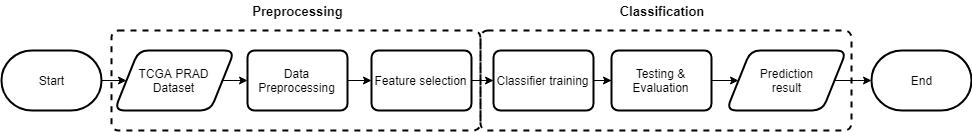
\includegraphics[width=1\linewidth]{system_design}
  \centering
  \caption{System Design}
  \label{fig:system_design}
\end{figure}

\subsection{Preprocessing}
Preprocessing needed to be performed to make the data usable for the training and testing process. First, we had to consolidate our data across hundreds of clinical pathology reports and DNA methylation profiles. After consolidation, we constructed a feature matrix in which each row corresponds to a patient and each column corresponds to a DNA methylation.
\par
We will also apply data normalization to each column and we will using Principal Component Analysis (PCA) as feature selection algorithm to eliminate the useless DNA methylation and reduce the search space.

\subsection{Classification}

This project perform on several classifier algorithms that proven give good result on many cases \cite{three} :
\begin{enumerate}
\item K-Nearest Neighbor (KNN)
\item Support Vector Machine (SVM)
\item Multilayer Perceptron (MLP)
\end{enumerate}

This project will finding a model that has the maximum classification accuracy, given by the Equation \ref{eq:1}, where $y_{i}'$ is the predicted label for instance $i$, $y$ is the true label for instance $i$. $I$ is an indicator function, if the statement is true, it will return $1$, and vice-versa.

\begin{equation} \label{eq:1}
accuracy =  \frac{1}{n}  \sum_{i=1}^n  I(y_{i}' = y_{i})
\end{equation}

\section{Experiments}
\begin{lstlisting}[language=Python]
import numpy as np
 
def incmatrix(genl1,genl2):
    m = len(genl1)
    n = len(genl2)
    M = None #to become the incidence matrix
    VT = np.zeros((n*m,1), int)  #dummy variable
 
    #compute the bitwise xor matrix
    M1 = bitxormatrix(genl1)
    M2 = np.triu(bitxormatrix(genl2),1) 
 
    for i in range(m-1):
        for j in range(i+1, m):
            [r,c] = np.where(M2 == M1[i,j])
            for k in range(len(r)):
                VT[(i)*n + r[k]] = 1;
                VT[(i)*n + c[k]] = 1;
                VT[(j)*n + r[k]] = 1;
                VT[(j)*n + c[k]] = 1;
 
                if M is None:
                    M = np.copy(VT)
                else:
                    M = np.concatenate((M, VT), 1)
 
                VT = np.zeros((n*m,1), int)
 
    return M
\end{lstlisting}

\section{Conclusion}

\begin{thebibliography}{1}
\bibitem{five} Ilir Agalliu, Robert Gern, Suzanne Leanza, and Robert D. Burk. 2009. {\em Associations of High-Grade Prostate Cancer with BRCA1 and BRCA2 Founder Mutations.} Clinical Cancer Research. Vol. 15, No. 3.
\bibitem{one} Hao, Xiaoke, et al. {\em DNA methylation markers for diagnosis and prognosis of common cancers.} Proceedings of the National Academy of Sciences 114.28 (2017): 7414-7419.
\bibitem{two} Genome.ifmo.ru. (2018). TCGA PRAD Dataset. [online] Available at: {\em https://genome.ifmo.ru/files/software/phantasus/tcga/PRAD/ } [Accessed 29 Nov. 2018].
\bibitem{three} Cancer.sanger.ac.uk. (2018). Cancer Gene Census. [online] Available at: {\em https://cancer.sanger.ac.uk/census } [Accessed 29 Nov. 2018].
\bibitem{four} Civicdb.org. (2018). CIViC - Clinical Interpretations of Variants in Cancer. [online] Available at: {\em https://civicdb.org/releases } [Accessed 29 Nov. 2018].
\end{thebibliography}
\end{document}